\part{Evaluation et Réalisation}
\label{part:evaluation-et-realisation}
\chapter{Evaluation du projet}
Ce chapitre traite de l’organisation et de la gestion du projet, en analysant
les éléments clés nécessaires à une évaluation efficace.

\section{Organisation du projet}
L’organisation du projet implique la définition des rôles, des responsabilités
et des processus de travail. Une structure organisationnelle claire facilite
la coordination et la communication entre les membres de l’équipe, assurant
ainsi une progression harmonieuse du projet.

% Dans le cadre de ce projet, l’organisation est structurée autour de deux
% principaux processus : le processus de développement et le processus de
% validation.
%
% \begin{table}[htbp]
%   \centering
%   \begin{tabularx}{\textwidth}{|l|X|}
%     \hline
%     \textbf{Processus} & \textbf{Phases} \\ \hline
%     \multirow{4}{*}{Développement} & Analyse des besoins : Définir les fonctionnalités nécessaires à la création collaborative et au partage d’arbres généalogiques. \\
%      & Conception : Concevoir l'architecture logicielle de la solution, ainsi que l'interface utilisateur pour le web et le mobile. \\
%      & Développement : Implémenter les fonctionnalités selon les spécifications définies lors de l'analyse et de la conception. \\
%      & Tests : Réaliser des tests unitaires et d'intégration pour garantir le bon fonctionnement de l'application. \\ \hline
%     \multirow{2}{*}{Validation} & Vérification : Vérifier que les fonctionnalités implémentées répondent aux besoins et aux spécifications du projet. \\
%      & Validation : Valider l'application avec les utilisateurs finaux pour recueillir leurs retours et effectuer les ajustements nécessaires. \\ \hline
%   \end{tabularx}
%   \caption{Organisation du projet}
% \end{table}

\section{Intervenant}

\begin{table}[htbp]
  \centering
  \begin{tabularx}{\textwidth}{|l|l|X|}
    \hline
    \textbf{Intervenants} & \textbf{Fonctions} & \textbf{Rôles} \\ \hline
    M. Christopher BANDZOUZI & Ingénieur Informaticien & Directeur de projet  \\ \hline
    M. Samuel Exaucé NANDI & Etudiant & Réalisateur \\ \hline
    M. Dieu-Veille Frédy ONIANGUE-DESO & Etudiant & Réalisateur \\ \hline
    Me. Rovélia MOUNTOU & Sécrétaire Mazala-Firm & Tutrice de stage \\ \hline
  \end{tabularx}
  \caption{Intervenants}
\end{table}

\section{Planification des tâches}
La planification des tâches consiste à décomposer le projet en activités
distinctes et à établir un calendrier pour leur réalisation. Elle permet de
suivre les progrès, de gérer les ressources efficacement et de
respecter les délais.

\begin{figure}[H]
  \centering
  % \begin{tabularx}{\textwidth}{|l|l|X|}
  %   \hline
  %   \textbf{Processus} & \textbf{Phases} & \textbf{Tâches} \\ \hline
  %   \multirow{2}{*}{Développement} & Analyse des besoins & - Étude des fonctionnalités nécessaires à la création collaborative et au partage d'arbres généalogiques. \\
  %    &  & - Identification des exigences de performance, de sécurité et de convivialité de la plateforme. \\ \cline{2-3}
  %   & Conception & - Conception de l'architecture logicielle de la solution, en mettant l'accent sur la scalabilité et la maintenabilité. \\
  %   &  & - Conception de l'interface utilisateur pour le web et le mobile, en tenant compte des principes de conception UX/UI. \\ \cline{2-3}
  %   & Développement & - Implémentation des fonctionnalités de création collaborative d'arbres généalogiques sur la plateforme web. \\
  %   &  & - Développement des fonctionnalités de partage et de visualisation des arbres généalogiques sur les applications mobiles. \\ \cline{2-3}
  %   & Tests & - Réalisation de tests unitaires et d'intégration pour garantir le bon fonctionnement des fonctionnalités développées. \\
  %   &  & - Tests de performance pour évaluer la réactivité et la scalabilité de la plateforme. \\ \hline
  %   \multirow{2}{*}{Déploiement} & Mise en production & - Configuration des serveurs et déploiement de l'application web Next.js sur un environnement de production sécurisé. \\
  %   &  & - Publication des applications mobiles sur les stores (App Store et Google Play) après une phase de tests approfondis. \\ \cline{2-3}
  %   & Formation & - Formation des utilisateurs finaux à l'utilisation de la plateforme, en mettant l'accent sur les fonctionnalités clés et les bonnes pratiques. \\
  %   &  & - Documentation complète de la plateforme pour une référence ultérieure. \\ \hline
  %   \multirow{2}{*}{Suivi} & Maintenance & - Surveillance continue de la plateforme pour détecter et corriger les éventuels problèmes de performance ou de sécurité. \\
  %   &  & - Mise à jour régulière de la plateforme avec de nouvelles fonctionnalités et correctifs de bugs. \\ \hline
  % \end{tabularx}
  % \caption{Planification des tâches}
  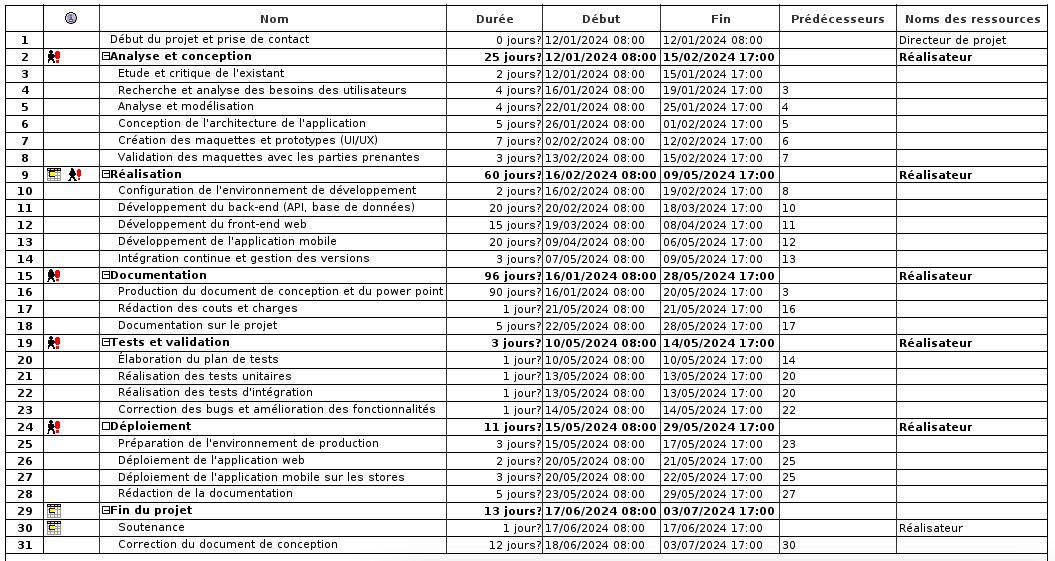
\includegraphics[width=1\textwidth]{capture/task.png}
  \caption{Planification des tâches}
\end{figure}


\section{Diagramme de Gantt}
Le diagramme de Gantt est un outil visuel de gestion de projet qui affiche les
tâches à accomplir sur une ligne de temps. Il permet de suivre les progrès,
d’identifier les dépendances entre les tâches et de prévoir les éventuels retards.

\newpage
% \begin{landscape}
%  \begin{sidewaysfigure}
%   \begin{ganttchart}[
%     hgrid,
%     vgrid,
%     x unit=0.5cm,
%     y unit title=0.7cm, % Augmenter légèrement la hauteur de chaque unité en titre
%     y unit chart=0.7cm, % Augmenter légèrement la hauteur de chaque unité en charte
%     time slot format=isodate,
%     title/.append style={draw=none, fill=gray!30},
%     title label font=\sffamily\bfseries\footnotesize,
%     title height=1,
%     title label anchor/.style={below=-1.6ex},
%     include title in canvas=false,
%     bar label font=\small,
%     bar label node/.append style={align=left},
%     bar/.append style={draw=none, fill=black!63},
%     bar height=0.6,
%     bar top shift=0.2,
%     group top shift=0.4,
%     group height=0.2,
%     group peaks width=0.2,
%     group peaks height=0.2,
%     group peaks tip position=0,
%     group label node/.append style={align=left}
%   ]{2024-05-01}{2024-07-31}
%
%   \gantttitlecalendar{month=shortname} \\
%
%   \ganttgroup{Phase 1}{2024-05-01}{2024-05-31} \\
%   \ganttbar{Task 1}{2024-05-01}{2024-05-15} \\
%   \ganttbar{Task 2}{2024-05-16}{2024-05-31} \\
%
%   \ganttgroup{Phase 2}{2024-06-01}{2024-06-30} \\
%   \ganttbar{Task 3}{2024-06-01}{2024-06-15} \\
%   \ganttbar{Task 4}{2024-06-16}{2024-06-30} \\
%
% \end{ganttchart}
% \end{sidewaysfigure}

% \newgantttimeslotformat{stardate}{%
%   \def\decomposestardate##1.##2\relax{%
%     \def\stardateyear{##1}\def\stardateday{##2}%
%   }%
%   \decomposestardate#1\relax%
%   \pgfcalendardatetojulian{\stardateyear-01-01}{#2}%
%   \advance#2 by-1\relax%
%   \advance#2 by\stardateday\relax%
% }

% \begin{ganttchart}[
%   hgrid,
%   vgrid,
%   time slot format=stardate
%   ]{2259.55}{2259.67}
%   \gantttitlecalendar{year, month=name, week} \\
% \end{ganttchart}

% \begin{ganttchart}[
%     hgrid style/.style={black, dotted},
%     vgrid={*6{black,dotted}, *1{black, dashed}},
%     x unit=3mm,
%     y unit chart=9mm,
%     y unit title=12mm,
%     time slot format=isodate,
%     group label font=\bfseries \Large,
%     link/.style={->, thick}
%     ]{2024-01-01}{2024-06-30}
%
%     % Headers
%     \gantttitlecalendar{year, month=name, week}\\
%
%     % Groupe Analyse des besoins
%     \ganttgroup[
%         group/.append style={fill=orange}
%     ]{Analyse des besoins}{2024-01-01}{2024-02-28} \\ [grid]
%     \ganttorangebar[
%         name=EtudeFonctionnalites
%     ]{Étude des fonctionnalités}{2024-01-01}{2024-01-31} \\ [grid]
%     \ganttorangebar[
%         name=IdentificationExigences
%     ]{Identification des exigences}{2024-01-15}{2024-02-28} \\ [grid]
%
%     % Groupe Conception
%     \ganttgroup[
%         group/.append style={fill=blue}
%     ]{Conception}{2024-02-01}{2024-03-31} \\ [grid]
%     \ganttbluebar[
%         name=ConceptionArchitecture
%     ]{Conception de l’architecture}{2024-02-01}{2024-02-28} \\ [grid]
%     \ganttbluebar[
%         name=ConceptionInterface
%     ]{Conception de l’interface}{2024-03-01}{2024-03-31} \\ [grid]
%
%     % Groupe Développement
%     \ganttgroup[
%         group/.append style={fill=green}
%     ]{Développement}{2024-03-01}{2024-04-30} \\ [grid]
%     \ganttgreenbar[
%         name=ImplementationFonctionnalites
%     ]{Implémentation des fonctionnalités}{2024-03-01}{2024-03-31} \\ [grid]
%     \ganttgreenbar[
%         name=DeveloppementFonctionnalites
%     ]{Développement des fonctionnalités}{2024-04-01}{2024-04-30} \\ [grid]
%
%     % Groupe Tests
%     \ganttgroup[
%         group/.append style={fill=red}
%     ]{Tests}{2024-04-01}{2024-05-31} \\ [grid]
%     \ganttredbar[
%         name=TestsUnitaires
%     ]{Tests unitaires et d’intégration}{2024-04-01}{2024-04-30} \\ [grid]
%     \ganttredbar[
%         name=TestsPerformance
%     ]{Tests de performance}{2024-05-01}{2024-05-31} \\ [grid]
%
%     % Groupe Mise en production
%     \ganttgroup[
%         group/.append style={fill=purple}
%     ]{Mise en production}{2024-05-01}{2024-05-31} \\ [grid]
%     \ganttpurplebar[
%         name=ConfigurationServeurs
%     ]{Configuration des serveurs}{2024-05-01}{2024-05-15} \\ [grid]
%     \ganttpurplebar[
%         name=PublicationApplications
%     ]{Publication des applications}{2024-05-16}{2024-05-31} \\ [grid]
%
%     % Groupe Formation
%     \ganttgroup[
%         group/.append style={fill=brown}
%     ]{Formation}{2024-05-15}{2024-06-30} \\ [grid]
%     \ganttbrownbar[
%         name=FormationUtilisateurs
%     ]{Formation des utilisateurs}{2024-05-15}{2024-05-31} \\ [grid]
%     \ganttbrownbar[
%         name=DocumentationComplete
%     ]{Documentation complète}{2024-06-01}{2024-06-30} \\ [grid]
%
%     % Groupe Maintenance
%     \ganttgroup[
%         group/.append style={fill=gray}
%     ]{Maintenance}{2024-06-01}{2024-06-30} \\ [grid]
%     \ganttgraybar[
%         name=SurveillanceContinue
%     ]{Surveillance continue}{2024-06-01}{2024-06-15} \\ [grid]
%     \ganttgraybar[
%         name=MisesAJour
%     ]{Mises à jour régulières}{2024-06-16}{2024-06-30} \\ [grid]
%
%     % Links
%     \ganttlink[link mid=0.75]{EtudeFonctionnalites}{ConceptionArchitecture}
%     \ganttlink[link mid=0.75]{IdentificationExigences}{ConceptionInterface}
%     \ganttlink[link mid=0.75]{ConceptionArchitecture}{ImplementationFonctionnalites}
%     \ganttlink[link mid=0.75]{ConceptionInterface}{DeveloppementFonctionnalites}
%     \ganttlink[link mid=0.75]{ImplementationFonctionnalites}{TestsUnitaires}
%     \ganttlink[link mid=0.75]{DeveloppementFonctionnalites}{TestsPerformance}
%     \ganttlink[link mid=0.75]{TestsUnitaires}{ConfigurationServeurs}
%     \ganttlink[link mid=0.75]{TestsPerformance}{PublicationApplications}
%     \ganttlink[link mid=0.75]{PublicationApplications}{FormationUtilisateurs}
%     \ganttlink[link mid=0.75]{FormationUtilisateurs}{DocumentationComplete}
%     \ganttlink[link mid=0.75]{DocumentationComplete}{SurveillanceContinue}
%     \ganttlink[link mid=0.75]{SurveillanceContinue}{MisesAJour}
%
% \end{ganttchart}

\begin{figure}[H]
  \centering
  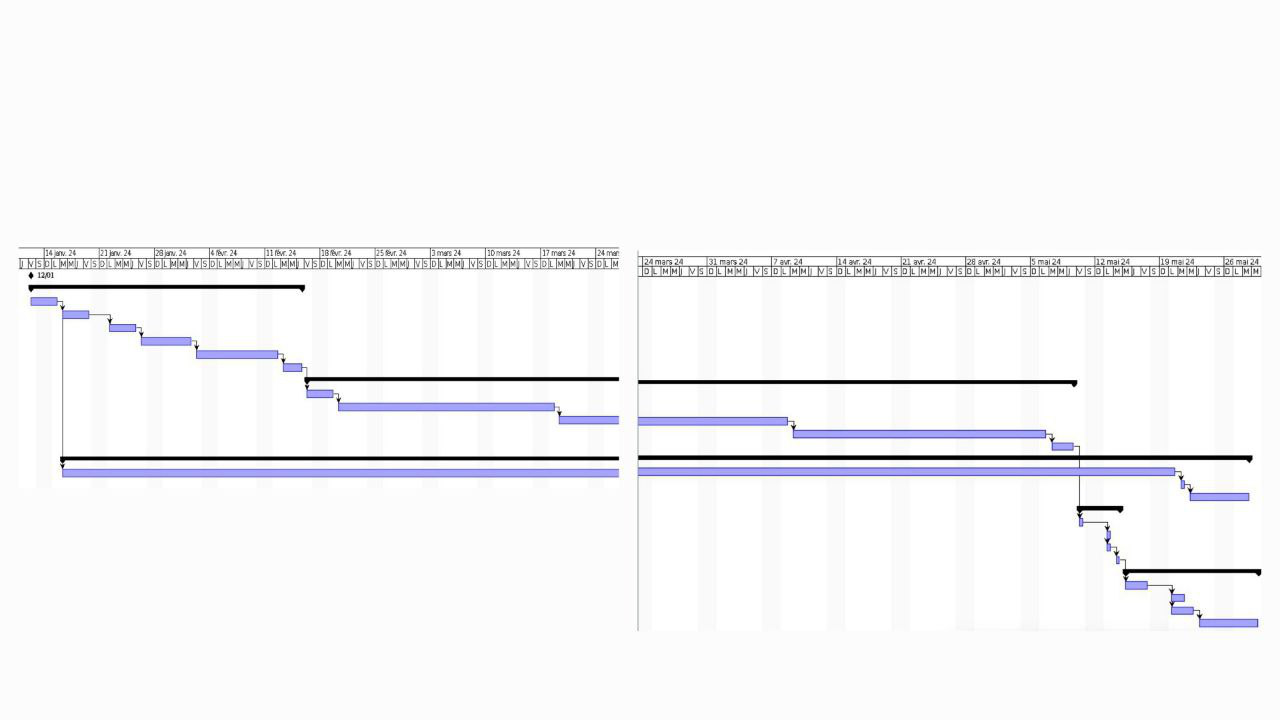
\includegraphics[width=1\textwidth]{capture/gantt.png}
  \caption{Diagramme de Gantt}
\end{figure}



\section{Estimation des charges}
L’estimation des charges implique de calculer le temps et les ressources
nécessaires pour accomplir chacune des tâches du projet.
Des estimations précises sont essentielles pour la planification budgétaire et
la gestion des ressources humaines.


\begin{table}[htbp]
  \centering
  \begin{tabular}{|l|c|c|}
    \hline
    \textbf{Outil et besoin} & \textbf{Quantité} & \textbf{Prix} \\ \hline
    \LaTeX & 1 & 0 FCFA  \\ \hline
    TypeScript & 1 & 0 FCFA  \\ \hline
    Next.js & 1 & 0 FCFA  \\ \hline
    Capacitor & 1 & 0 FCFA  \\ \hline
    PostgreSQL & 1 & 0 FCFA  \\ \hline
    Docker & 1 & 0 FCFA  \\ \hline
    Git & 1 & 0 FCFA  \\ \hline
    GitHub & 2 & 0 FCFA  \\ \hline
    Neovim & 1 & 0 FCFA  \\ \hline
    VSCodium & 1 & 0 FCFA  \\ \hline
    Figma & 1 & 0 FCFA  \\ \hline
    PC Portable & 2 & 400 000 FCFA  \\ \hline
    Connexion internet & 6 & 25 000 FCFA \\ \hline
    Réalisateurs & 2 & 4 000 000 FCFA \\ \hline
    \multicolumn{2}{|l|}{\textbf{Total}} & \textbf{8 950 000 FCFA} \\ \hline
  \end{tabular}
  \caption{Estimation des charges}
\end{table}

\chapter{Les outils et techniques utilisés}
Ce chapitre présente les outils et les techniques utilisées pour développer
et gérer le projet.

\section{Présentation des techniques}
Les techniques utilisées dans le cadre de ce projet sont les suivantes :

  \textbf{ {Développement Web et Mobile}}

    Pour le développement de la plateforme, nous avons utilisé des techniques
    modernes adaptées au web et aux applications mobiles.
    \begin {itemize}
  \item \textbf{{Next.js}}
    Next.js est un framework React qui permet de créer des applications web côté
    serveur (SSR) et des applications statiques (SSG). Il offre des fonctionnalités
    avancées telles que le rendu côté serveur, le pré-rendu statique, et une
    gestion automatique des routes, ce qui améliore la performance et le
    SEO des applications web.

  \item \textbf{{Capacitor}}
    Capacitor crée un environnement de développement pour les applications en
    transformant les applications web en applications mobiles natives avec
    JavaScript, HTML et CSS.

\end{itemize}

\textbf{{Base de Données}}

  Pour stocker les données de l'application, nous avons utilisé une base de
  données relationnelle PostgreSQL, qui offre des fonctionnalités avancées
  telles que la conformité ACID, la gestion des transactions, et la prise en
  charge de données complexes.

\textbf{{Sécurité}}

  La sécurité est un aspect crucial du développement de la plateforme. Nous
  avons mis en place plusieurs techniques de sécurité pour protéger les données
  des utilisateurs.
  \begin{itemize}
    \item \textbf{{Authentification et Autorisation}}

      Nous avons utilisé un système de session lié à la base de donnée pour
      l'authentification. Les autorisation, pour sécuriser les accès
      à l'application et aux API sont fait par rapport à ces sessions.

    \item \textbf{{Chiffrement des Données}}

      Toutes les communications entre les clients et le serveur sont chiffrées
      en utilisant TLS (Transport Layer Security), garantissant que les données
      transmises restent confidentielles et intactes.
  \end{itemize}

\textbf{Gestion de Projet}

Pour la gestion du projet, nous avons utilisé la méthode objet, qui permet
d'organiser les tâches en fonction de leur importance et de leur priorité.


\section{Présentation des outils}
Les outils utilisés dans le cadre de ce projet sont les suivants :

\textbf{Outils de Développement}
\begin{itemize}
  \item \textbf{Neovim}

    Neovim est un éditeur de texte puissant et extensible, adapté au
    développement de logiciels. Il offre des fonctionnalités avancées telles
    que la coloration syntaxique, la complétion automatique, et la gestion
    des plugins, ce qui améliore la productivité des développeurs.

    \begin{figure}[H]
      \centering
      
\includegraphics[width=0.5\textwidth]{images/Neovim-logo.png}
      \caption{Logo Neovim}
    \end{figure}

  \item \textbf{VSCodium}

    VSCodium est un éditeur de code open-source basé sur Visual Studio Code,
    \begin{figure}[H]
      \centering
      
\includegraphics[width=1.0in, height=1.0in]{images/codium_cnl.png}
      \caption{Logo VSCodium}
    \end{figure}
\end{itemize}

\textbf{Frameworks et Bibliothèques}
\begin{itemize}
  \item \textbf{React}

    React est la bibliothèque JavaScript principale utilisée pour construire
    les interfaces utilisateur de la plateforme web.

  \item \textbf{Capacitor}

    Capacitor est un framework qui permet de créer des applications mobiles
    multiplateformes avec des technologies web comme React,  Vue et bien d'autre.
    Il offre des fonctionnalités telles que l'accès aux API natives, la gestion
    des plugins, et la compatibilité avec les stores d'applications.

    \begin{figure}[H]
      \centering
      
\includegraphics[width=0.5\textwidth]{images/Capacitor-JS-2375506976.png}
      \caption{Logo Capacitor}
    \end{figure}

  \item \textbf{Next.js}

    Next.js est le framework React utilisé pour le développement côté serveur
    et la génération de sites statiques de la partie web de la plateforme.

    \begin{figure}[H]
      \centering
      
\includegraphics[width=0.5\textwidth]{images/Nextjs-logo.svg.png}
      \caption{Logo Next.js}
    \end{figure}

  % \item \textbf{Expo}
  %
  %   Expo est la plateforme utilisée pour le développement et le déploiement
  %   des applications mobiles, en fournissant un ensemble d'outils et de
  %   services pour React Native.
  %
  %   \begin{figure}[H]
  %     \centering
  %     
\includegraphics[width=0.5\textwidth]{images/logo-wordmark.png}
  %     \caption{Logo Expo}
  %   \end{figure}

  \item \textbf{shadcn/ui}

    shadcn/ui est une bibliothèque de composants React réutilisables, qui
    permet de créer des interfaces utilisateur cohérentes et esthétiques.
\end{itemize}

\textbf{Outils de Contrôle de Version}
\begin{itemize}
  \item \textbf{Git}

    Git est le système de contrôle de version distribué utilisé pour suivre
    les modifications du code source et faciliter la collaboration entre les
    développeurs.

    \begin{figure}[H]
      \centering
      
\includegraphics[width=0.3\textwidth]{images/Git-logo.svg.png}
      \caption{Logo Git}
    \end{figure}

  \item \textbf{GitHub}

    GitHub est la plateforme utilisée pour héberger le code source et faciliter
    la collaboration via des fonctionnalités comme les pull requests et les
    revues de code.

    \begin{figure}[H]
      \centering
      
\includegraphics[width=1.0in, height=1.0in]{images/GitHub_Invertocat_Logo.svg.png}
      \caption{Logo GitHub}
    \end{figure}
\end{itemize}

\textbf{Outils de Conception}
\begin{itemize}
  \item \textbf{Figma}

    Figma est l'outil de conception utilisé pour créer les maquettes et les
    prototypes de l'interface utilisateur de la plateforme, en facilitant la
    collaboration et le partage des designs.

    \begin{figure}[H]
      \centering
      
\includegraphics[width=1.0in, height=1.2in]{images/800px-Figma-logo.svg.png}
      \caption{Logo Figma}
    \end{figure}

  \item \textbf{\LaTeX}

    \LaTeX est un système de composition de documents utilisé pour rédiger les
    documentations techniques et les rapports. Il offre une mise en
    page professionnelle et une gestion avancée des références. Il permet
    également de créer des diagrammes UML et de toute sorte.

    \begin{figure}[H]
      \centering
      
\includegraphics[width=0.5\textwidth]{images/LaTeX_project_logo_bird.svg.png}
      \caption{Logo \LaTeX}
    \end{figure}
\end{itemize}

\textbf{Outils de Base de Données}
\begin{itemize}
  \item \textbf{PostgreSQL}

    PostgreSQL est le système de gestion de base de données relationnelle
    utilisé pour stocker les données de l'application, en offrant des
    fonctionnalités avancées de gestion des données et de sécurité.

    \begin{figure}[H]
      \centering
      
\includegraphics[width=1.0in, height=1.0in]{images/Postgresql_elephant.svg.png}
      \caption{Logo PostgreSQL}
    \end{figure}

  \item \textbf{Prisma}

    Prisma est un \ac{ORM}  utilisé pour simplifier
    l'accès à la base de données PostgreSQL et faciliter les opérations de
    lecture et d'écriture des données.
    \begin{figure}[H]
      \centering
      
\includegraphics[width=1.0in, height=1.0in]{images/icons8-prisma-orm-500.png}
      \caption{Logo Prisma}
    \end{figure}

  \item \textbf{tRPC}

    tRPC est une bibliothèque de communication entre le client et le serveur
    qui facilite l'appel des API et la gestion des données de manière
    sécurisée et efficace.

    \begin{figure}[H]
      \centering
      
\includegraphics[width=0.5\textwidth]{images/trpc.png}
      \caption{Logo tRPC}
    \end{figure}
\end{itemize}

\textbf{Outils de Sécurité}
\begin{itemize}

  \item \textbf{TLS (Transport Layer Security)}

    TLS est utilisé pour chiffrer les communications entre les clients et le
    serveur, en garantissant la confidentialité et l'intégrité des
\end{itemize}

% \item \textbf{Outils de test}
%   \begin{itemize}
%     \item \textbf{Jest}
%
%       Jest est utilisé pour les tests unitaires et les tests d'intégration du
%       code JavaScript et TypeScript.
%
%     \item \textbf{React Testing Library}
%
%       React Testing Library est utilisée pour tester les composants React de
%       manière efficace et fiable.
%   \end{itemize}

\textbf{Outils de conteneurisation}
\begin{itemize}
  \item \textbf{Docker}

    Docker est utilisé pour créer des conteneurs légers et portables qui
    encapsulent les applications et leurs dépendances, facilitant le
    déploiement et la gestion des applications dans différents environnements.

    \begin{figure}[H]
      \centering
      
\includegraphics[width=0.5\textwidth]{images/Docker_logo.svg.png}
      \caption{Logo Docker}
    \end{figure}
\end{itemize}

\textbf{Outils de Déploiement}
\begin{itemize}
  \item \textbf{Vercel}

    Vercel est utilisé pour le déploiement et l'hébergement de la partie web
    de la plateforme développée avec Next.js.

    \begin{figure}[H]
      \centering
      
\includegraphics[width=0.5\textwidth]{images/Vercel_logo_black.svg.png}
      \caption{Logo Vercel}
    \end{figure}

  \item \textbf{AppFlow}

    AppFlow est utilisé pour le déploiement et la gestion des applications
    mobiles développées avec Capacitor, React Native et bien d'autre, en
    facilitant le processus de publication
    sur les stores d'applications.

    \begin{figure}[H]
      \centering
      
\includegraphics[width=0.3\textwidth]{images/AppFlow.png}
      \caption{Logo AppFlow}
    \end{figure}
\end{itemize}


\section{Les captures d'écrans}
Les captures d’écran illustrent visuellement les étapes importantes du
développement et l’interface utilisateur du produit final. Elles servent à
documenter le travail accompli et à fournir des exemples concrets de
l’application en action.

\begin{figure}[H]
  \centering
  
\includegraphics[width=1\textwidth]{./capture/home.png}
  \caption{Écran d'accueil sur l'application web}
\end{figure}

\begin{figure}[H]
  \centering
  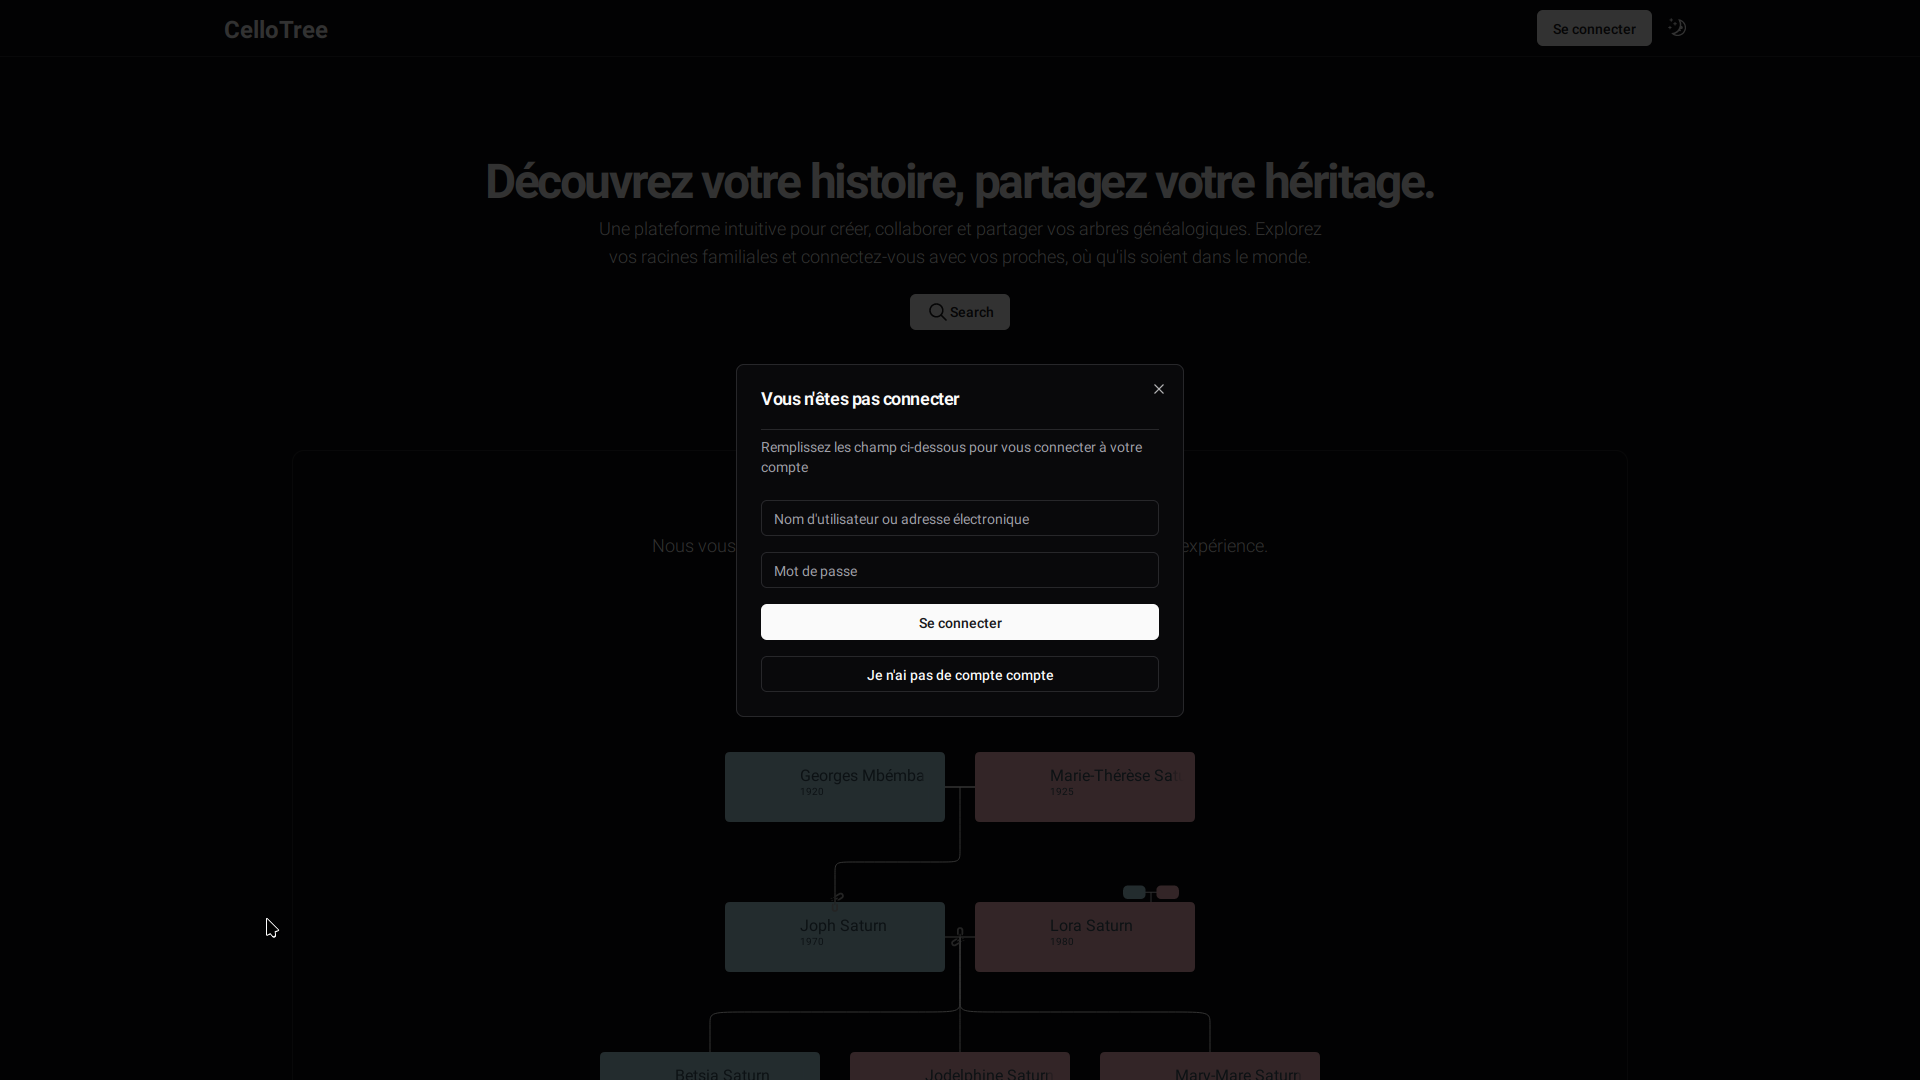
\includegraphics[width=1\textwidth]{capture/login.png}
  \caption{Écran de connexion sur l'application web}
\end{figure}

\begin{figure}[H]
  \centering
  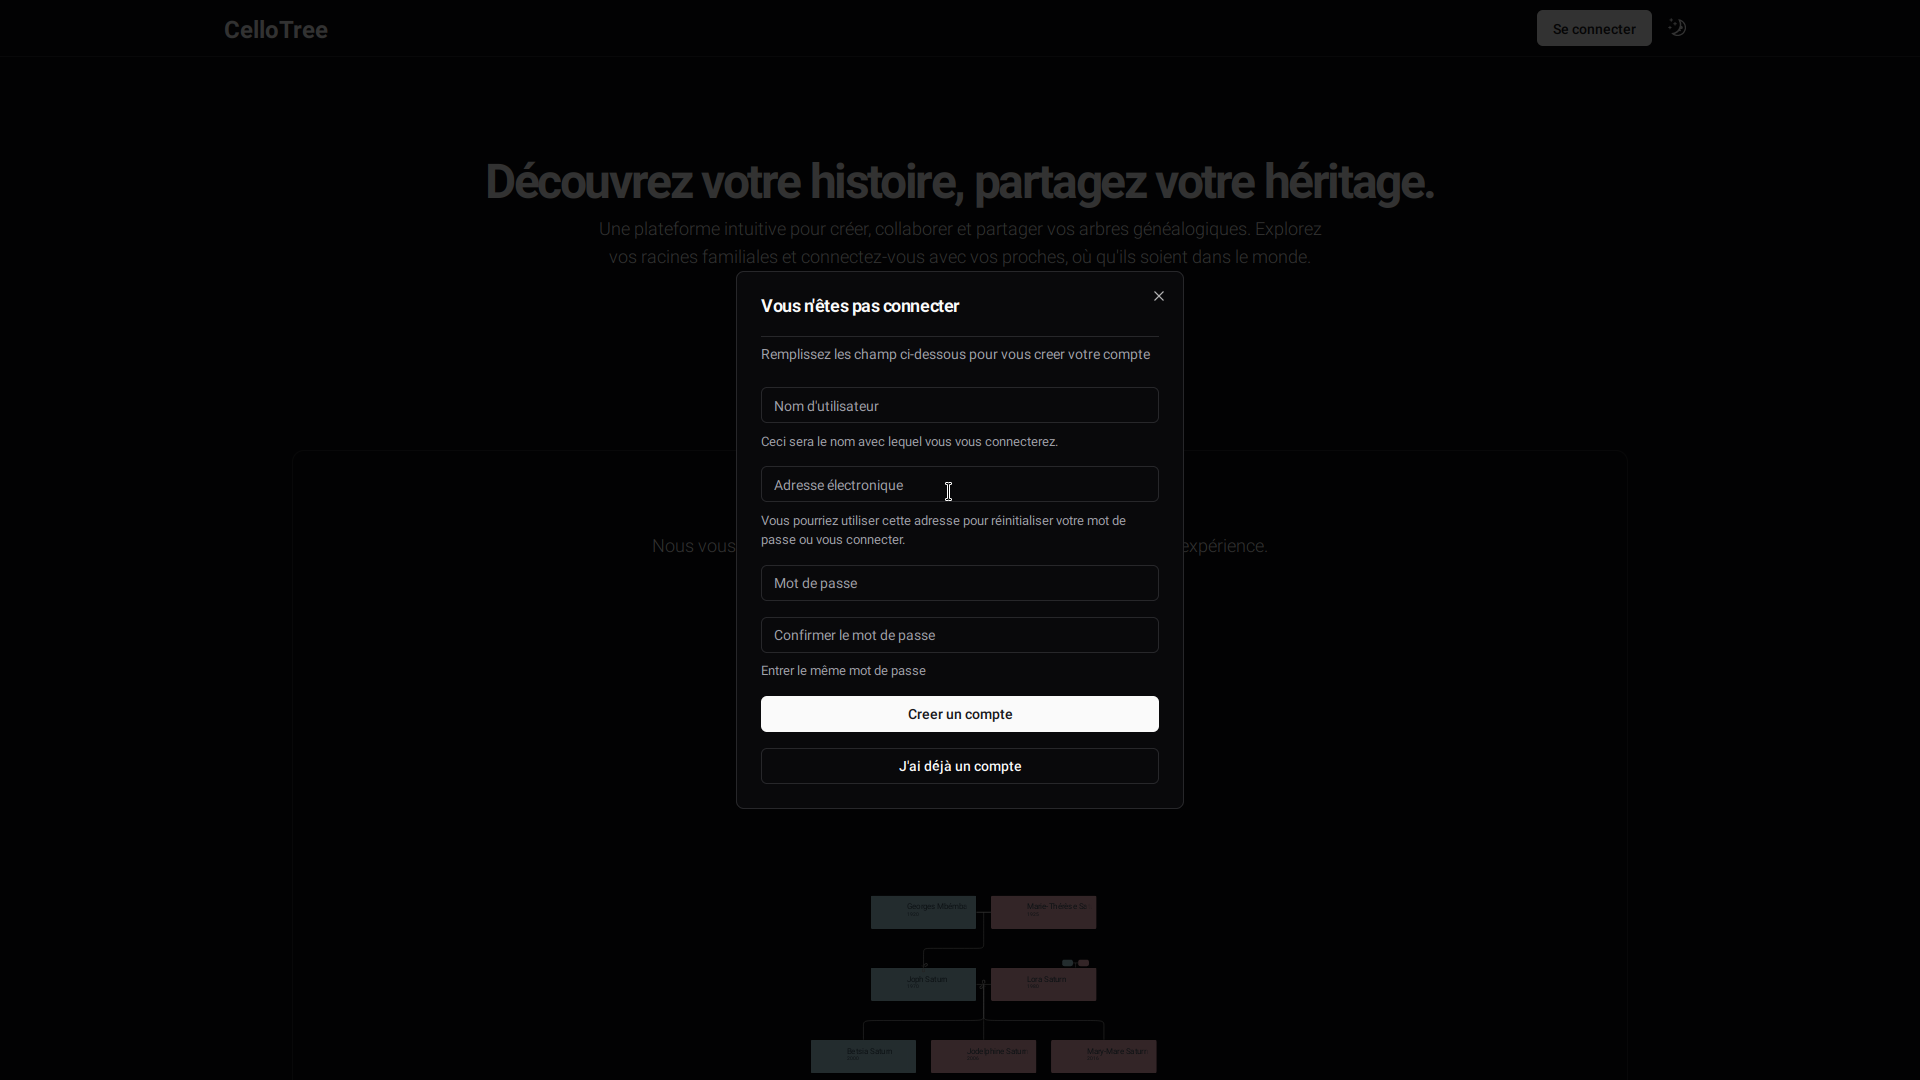
\includegraphics[width=1\textwidth]{capture/signup.png}
  \caption{Écran de création de compte sur l'application web}
\end{figure}

\begin{figure}[H]
  \centering
  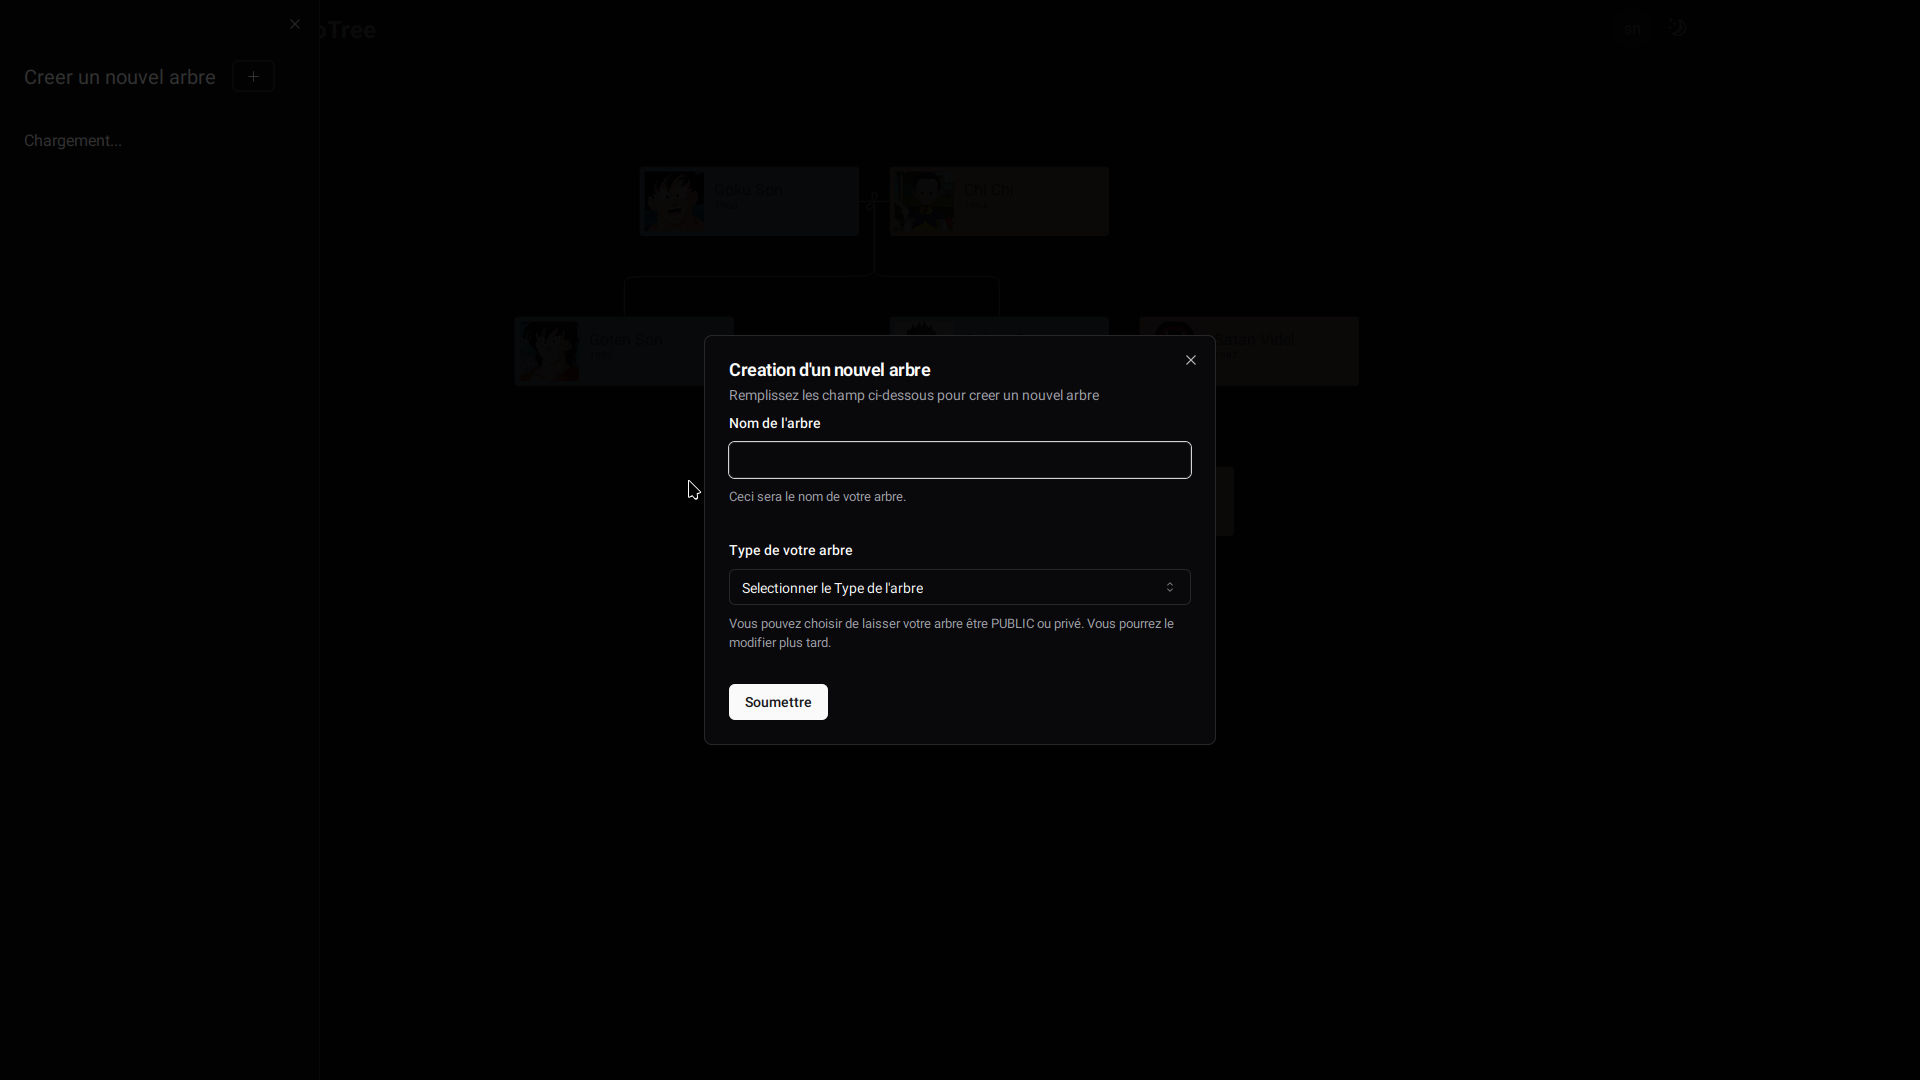
\includegraphics[width=1\textwidth]{capture/tree.png}
  \caption{Écran de création d'un arbre généalogique sur l'application web}
\end{figure}

\begin{figure}[H]
  \centering
  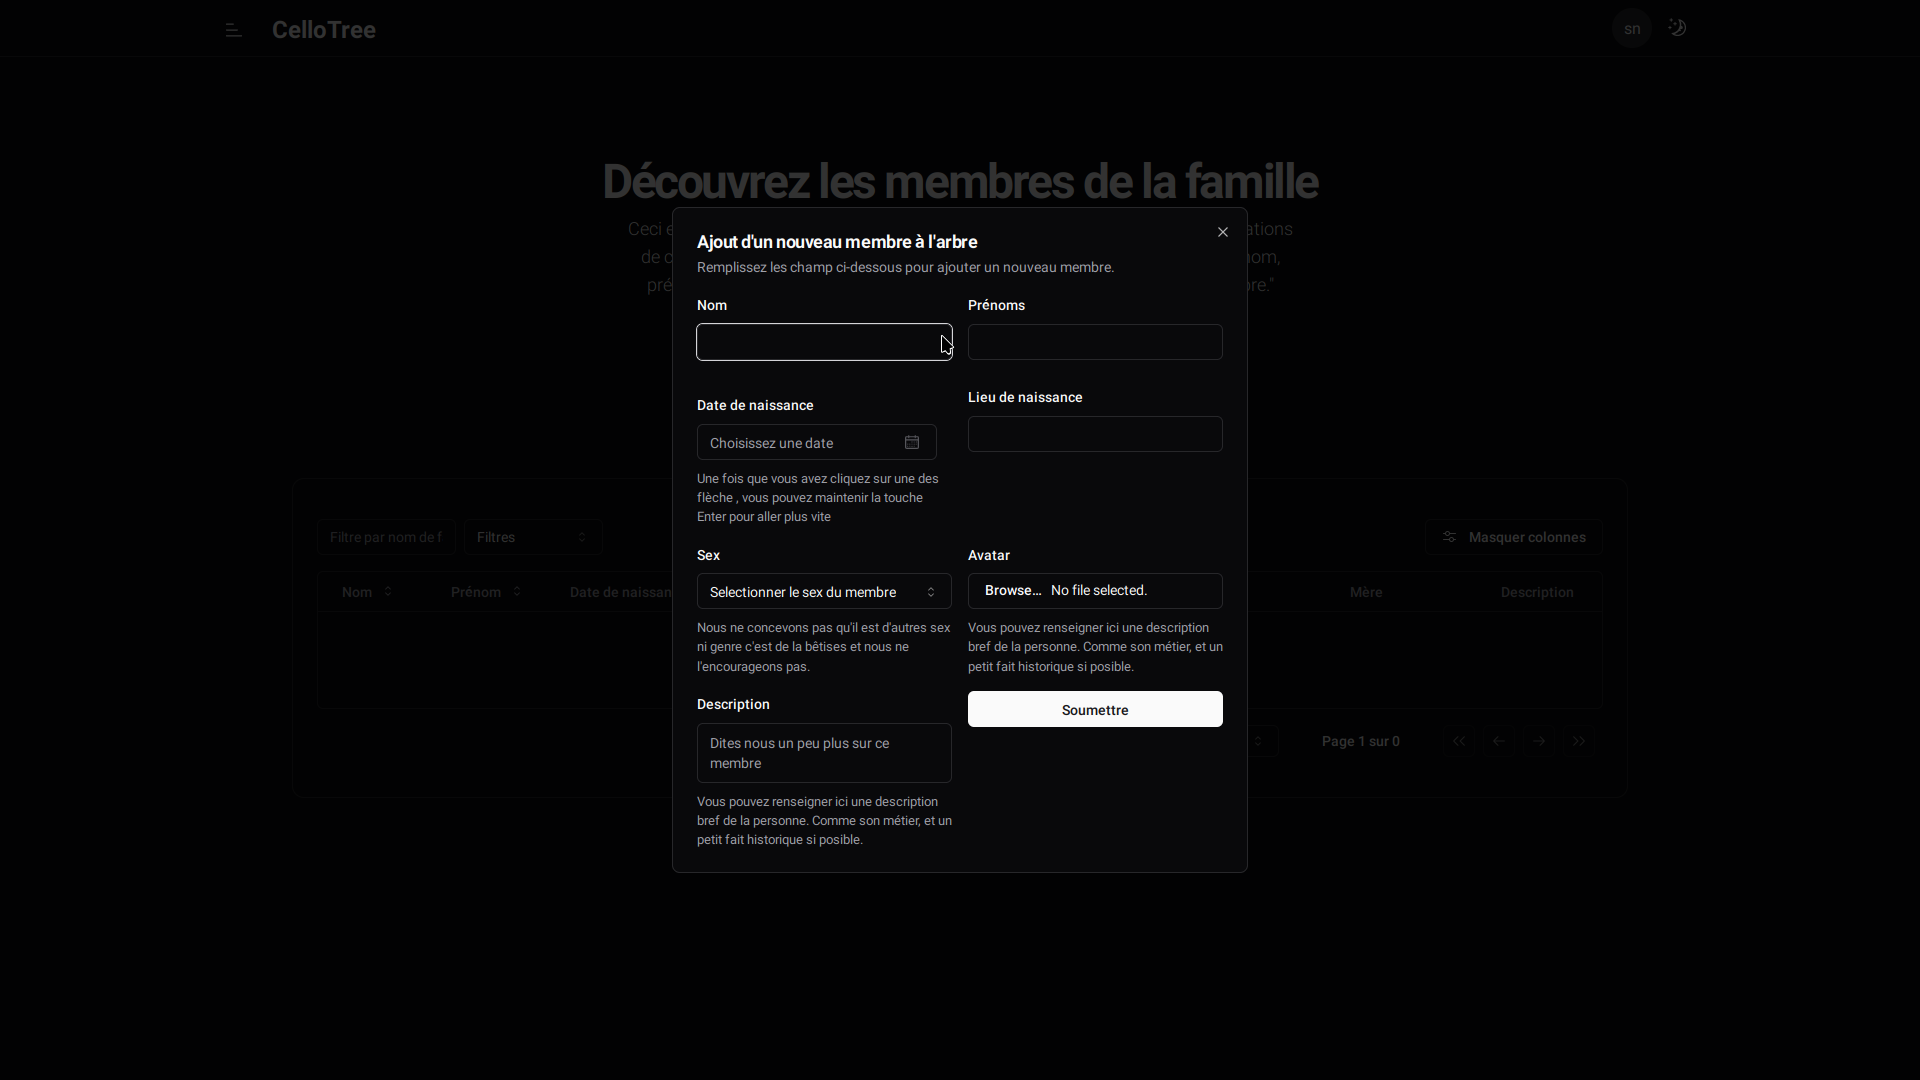
\includegraphics[width=1\textwidth]{capture/member.png}
  \caption{Écran d'ajout d'un membre à un généalogique sur l'application web}
\end{figure}

\begin{figure}[H]
  \centering
  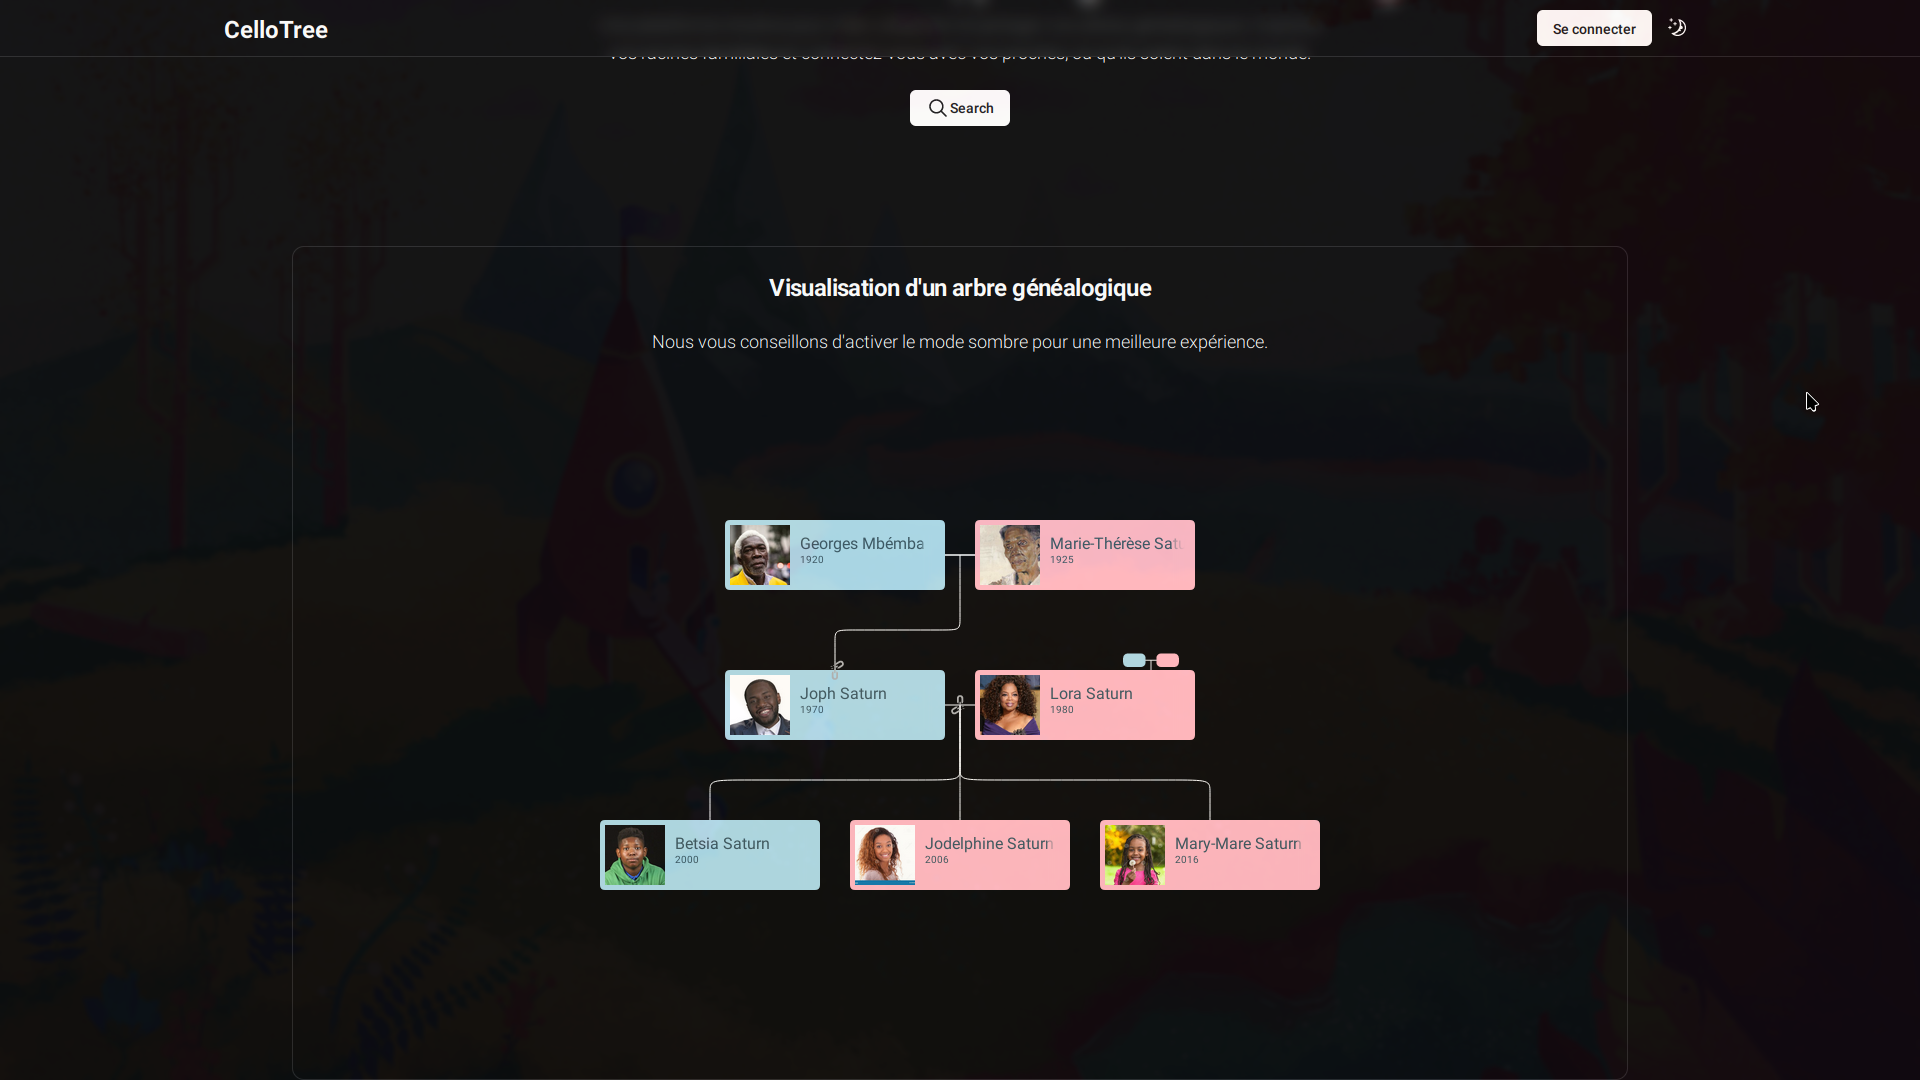
\includegraphics[width=1\textwidth]{capture/view.png}
  \caption{Écran de visualisation d'un arbre généalogique}
\end{figure}


\begin{figure}[H]
  \centering
  
\includegraphics[width=0.3\textwidth]{./capture/homem.png}
  \caption{Écran d'accueil sur l'application mobile}
\end{figure}


\begin{figure}[H]
  \centering
  
\includegraphics[width=0.3\textwidth]{capture/loginw.png}
\caption{Écran de connexion sur l'application mobile}
\end{figure}


\begin{figure}[H]
  \centering
  
\includegraphics[width=0.3\textwidth]{capture/signupw.png}
  \caption{Écran de création de compte sur l'application mobile}
\end{figure}


\begin{figure}[H]
  \centering
  
\includegraphics[width=0.3\textwidth]{capture/treem.png}
  \caption{Écran de création d'un arbre généalogique sur l'application mobile}
\end{figure}


\begin{figure}[H]
  \centering
  
\includegraphics[width=0.3\textwidth]{capture/memberm.png}
  \caption{Écran d'ajout d'un membre à un généalogique sur l'application mobile}
\end{figure}
